\chapter{Heritage of ice reservoirs}

\cleanchapterquote{Before the artificial glacier, we struggled to get any barley. But now we can grow many
	crops, even potatoes, which need to be planted earlier in the spring, but sell for much more money.
}{Tashi Tundup}{(A 76 year old farmer in Ladakh)}

Climate warming has resulted in retreat and thinning of mountain glaciers
\citep{ipccCrossChapterPaperMountains2022}. This has implications for water availability in river basins that
have considerable glacierized areas in their headwaters, such as \ac{HMA}. Glaciers in HMA provide an important
gradual release of water that is used by many people locally and downstream for irrigation, drinking water and
hydropower. Climate change in this densely populated region may have serious consequences for glacier melt water
supply to the rivers \citep{immerzeelImportanceVulnerabilityWorld2020}. In this context, the development of
water storage technologies is crucial to ensure continued sustenance of cryosphere-fed irrigation networks.

People in mountains have a history of developing nature-based solutions to live in a dangerous and dynamic
environment, which will be invaluable to learn from for future adaptation and mitigation measures. One such
technology developed by communities in Ladakh are \ac{AIRs}. These strategies involve augmenting their glacial
ice reservoirs with man-made ones that provide supplementary irrigation during the spring.

\begin{figure}[htb]
	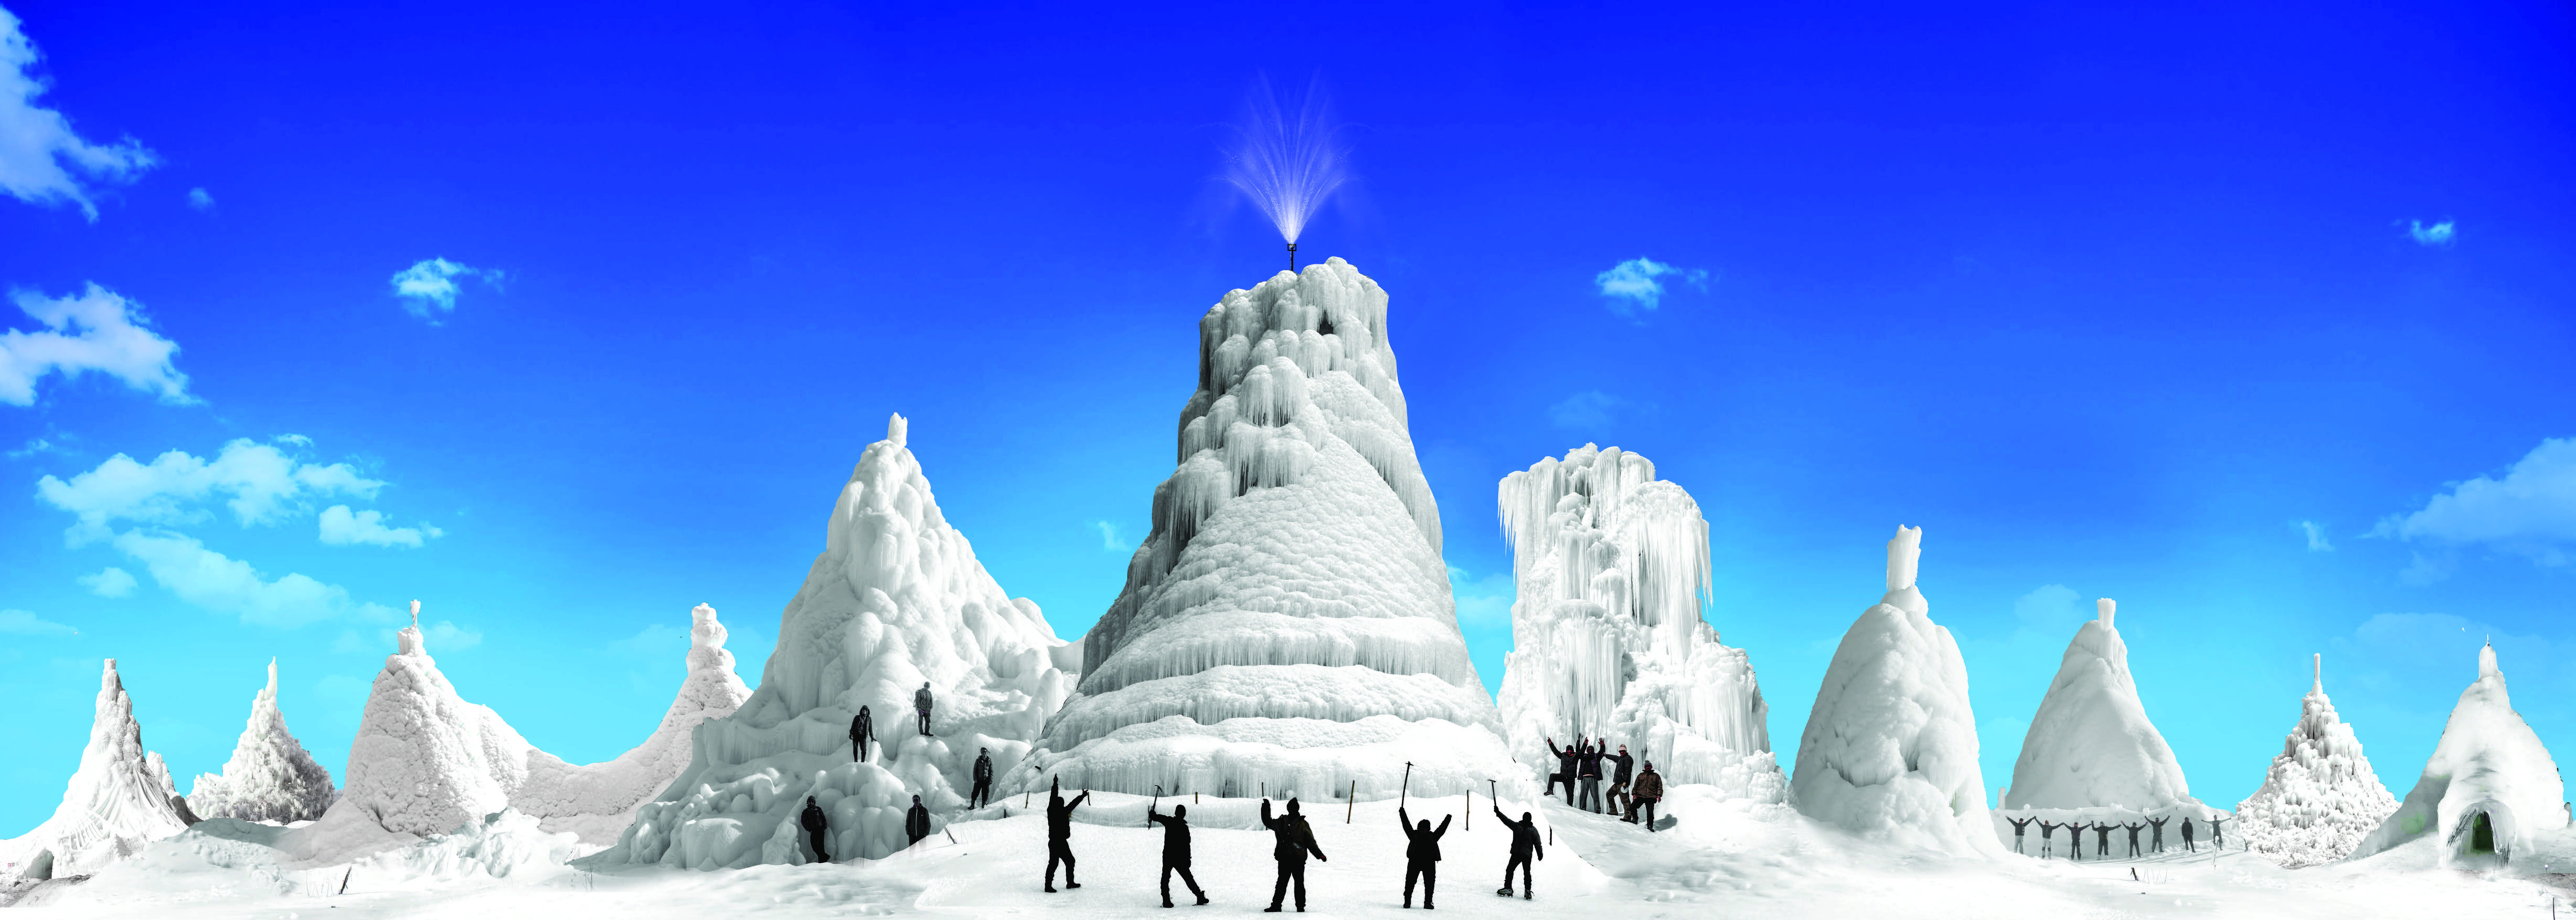
\includegraphics[width=\textwidth]{figs/AIRs_Ladakh}
	\caption{Compilation of AIRs built in different villages of Ladakh.}
	\label{fig:airs_ladakh}
\end{figure}

While these technologies have gained renewed attention as a strategy to increase water security, limited
scientific evidence exists about their potential hydrological contributions. AIR observations and investigations
date back to the mid-2000s \citep{tveitenGlacierGrowingLocal2007}. The vast majority have been published in the
2010s, mostly using qualitative methods. Because small-scale processes, complex feedbacks and non-linearities
govern their evolution, modelling the volume evolution of ice stupas is difficult and only feasible if backed up
with comprehensive datasets. Recent advances in glacial models and drones provide the opportunity to quantify
these surface processes using high-resolution data on volume changes of \ac{AIRs}. The main objective of the
thesis therefore was \textit{to increase understanding of volume dynamics of \ac{AIRs} in order to integrate
this tool in the water resource management strategy of mountain catchments}, with a specific focus on the
potential application of glacial models. This has been achieved by focusing on the following two specific
research questions:

\begin{enumerate}
  \item{What is the influence of construction location and fountain characteristics on ice stupa volume
    evolution?}
  \item{How can ice stupa fountain systems be engineered to reduce their water losses and maintenance efforts?}
\end{enumerate}

In this chapter, I synthesize the research presented in this thesis. I discuss the main findings, integrate them
in a broader perspective, and provide recommendations and a future outlook.

% In response, we conducted measurement campaigns using drones, flowmeters and weather stations on almost a dozen
% AIRs across two locations (India and Switzerland), over four winters (2019, 2020, 2021 and 2022) and using two
% different construction methods (traditional and automated). Each dataset contained information on the
% meteorological conditions, fountain characteristics and AIR volume evolution.

% The primary objective of this thesis was to improve our understanding of AIRs' response to changes in
% their construction location. The secondary objective was to propose automated construction strategies that reduce
% water losses and maintenance efforts.

\section{Conclusions}

\begin{figure}[htb]
	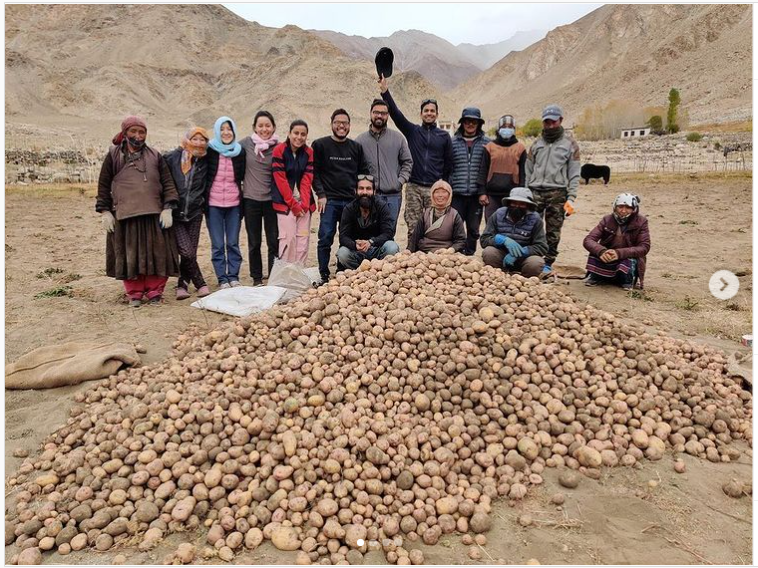
\includegraphics[width=\textwidth]{figs/Kullum_potatoes}
	\caption{One of the deserted villages in Ladakh where AIR meltwater supported a harvest of 1300 kg of
		potatoes in October 2021. (Picture credits: Icestupa Project)}
	\label{fig:kullum_potatoes}
\end{figure}

In paper I, an AIR model was designed to resolve surface processes and used to compare their volume evolution in
Indian Himalayas and the Swiss Alps. In paper II, the evolution of AIRs using different fountain scheduling
strategies were compared. In paper III, the possibility of sustaining artificial ice reservoirs perpetually was
explored. The methodology presented in this thesis accounts for variations in a location's meteorology and AIR
construction design. Although the approach is demonstrated on specific locations using fountain pipeline
systems, it can be extended to account for different construction strategies used in other locations. The
results of these papers can be summarised as follows:

\begin{enumerate}

	\item Volumes of ice stupas located in different regions may differ by an order of magnitude. The differences
	      could be attributed to the accelerated sublimation process in colder and drier regions.

	\item Water losses of ice stupas may be upto 80 \% due to excessive water input. However, water supply
	      management through fountain scheduling strategies can produce ice stupas of similar volumes while reducing up to
	      one-tenth of their water supply.

	\item Traditional construction systems demand significant maintenance efforts since they are prone to freezing
	      events in the fountain pipeline. However, automated construction systems can prevent these events to make the
	      construction process maintenance-free.

	\item There exist locations with favourable meteorological conditions that can sustain artificial ice reservoirs
	      perpetually.

\end{enumerate}


\section{Discussion}

\subsection{The state of ice stupa technology}

The thesis shows one strategy that can improve the water-use efficiency of AIRs. We chose this strategy because
it enables the use of the AIR model in a simple and effective manner. However, all these construction strategies are
limited by the tools they use, namely the fountain and the pipeline. The fountain nozzle design is crucial for
increasing the ice volume obtained. However, no methodology currently exists to rank the several fountain
nozzles used for construction. An ideal pipeline configuration could make this technology cheaper and
maintenance free. However, optimization of the pipeline material and diameters is yet to be performed---despite
the time lost on pipeline freezing events and the potential cost reduction with cheaper pipeline materials and
sizes. Therefore, we strongly encourage the engineering community to get involved and push the limits of the
cost-effectiveness, size, and survival duration of artificial ice reservoirs.

\subsection{Adaptation potential of glacierized catchments with AIRs}

Vanishing glaciers, natural hazards (like inundations, mudflows, and landslides), decreasing river discharge,
drying springs, next to shifts in precipitation patterns are apparent climate change impacts which affect
glacierized catchments.

In the Peruvian Andes, both water scarcity (low-flow water risk) and glacial lake outburst floods (high flow
water risks) could have important impacts on local population, infrastructure and economic activities
\citep{motschmannIntegratedAssessmentsWater2020}. For example, the estimated loss in annual wheat output due to
reduced glacial runoff would be to the tune of 18 million USD even in the low emission scenario of Quillcay catchment
of Peru \citep{motschmannLossesDamagesConnected2020}. Similarly, in the Stok catchment of Ladakh, glacial ice
reserves have shrunk by more than 18 \% in the past 16 years, leading to a decline in crop productivity
\citep{sohebSpatiotemporalQuantificationKey2022}.

AIRs can already buffer against low flow water risks in certain catchments. For example, ice
terraces in nearby valleys have been measured with areas up to 19 \% of the Stok glacier (0.8 $km^2$). With further technology
development, AIRs can also be used to mitigate high flow water risks. The glacial lakes of the Andes and
Himalayas can be siphoned to form AIRs in scale that last perpetually. Such AIRs can compound over the years to
become another source of perennial water supply for the respective catchments.

\subsection{Metrics to judge site suitability}

We propose two sets of guidelines to identify future construction sites at a regional and a local scale. These
suggestions are guided by the different case studies presented in this thesis and field experiences in
Ladakh over the past six winters.

\subsubsection{Regional scale}

\begin{enumerate}

	\item Minimum median monthly temperature less than $0 \degree C$.
	\item Water supply with median discharge rate more than $2\, l/min$.
	\item Terrain slope between water source and site greater than 20 m every km.

\end{enumerate}

\subsubsection{Local scale}

Given a valley or a region satisfying the above requirements, further selection of sites around the particular
water supply can be performed using the criterions below:

\begin{enumerate}
	\item Water source temperature is higher.
	\item Daylight hours are lower due to shadows.
	\item Altitude is higher.
\end{enumerate}

% \section{Model limitations and suggestions for improvement}
\subsection{Model development}

The COSISTUPA model developed in section \ref{sec:Cosistupa} should be used for future estimations for AIR
volume. This model needs to be extended so that it can account for future climate variability and produce
accurate meltwater predictions. Modelling the future is fundamentally different from simulating the past: In the
past the model serves as a tool for interpreting and best exploiting field measurements - and can be directly
constrained by them. Models for the future must understand climate variability to be able to yield realistic
projections. Almost all methodological steps in the modelling of future AIR runoff are subject to possible
enhancements, always bearing in mind that we will only know whether the effort led to an enhanced or even a
worsened performance, when we're old...

% \section{Model limitations and suggestions for improvement}

Model development is an art where subjective choices seek a balance between a model's simplicity and its
accuracy. Below we detail some of these choices and recommend strategies that shift this balance towards further
model accuracy.

\subsubsection{Quality and quantity of calibration and validation data sets}

The methodology used to acquire the radius, area and volume of \ac{AIRs} ( Appendix \ref{sec:drone_method}) from
each drone survey has several drawbacks. The calibration and validation process used has an inherent temporal
and spatial bias due to the following subjective choices:

\begin{itemize}
	\item \textbf{The number and timing of the drone surveys}. For example, among the five surveys of IN21 AIR, most of them were
	      conducted around early March when the AIR volume was near its maximum whereas the seven surveys of the CH21
	      location were more evenly spaced out in comparison. This observation bias occured due to logistical issues
	      in conducting measurements in regular intervals.

	\item \textbf{The meteorological conditions under which surveys were performed.} Particularly, precipitation events reduce DEM quality since
	      they create uniform snow surfaces over \ac{AIRs}. These surfaces do not allow the identification of features
	      that can be used to extract the radius and area of the AIR.

\end{itemize}

Thus, the quality of AIR validation is severely limited by the high uncertainties attached with the drone
processing methodology.

This limitation can be overcome by extending the model validation set using two measurement approaches. First,
we suggest measuring daily AIR meltwater quantities. Accuracy of this validation method depends on the wind
speeds of the location but can be improved if the terrain is made waterproof and oriented so that most of the
AIR runoff can be collected. 

Second, we suggest conducting \ac{GPR} surveys. Ice is very transparent to \ac{GPR} signals, allowing tremendous
penetration. \ac{GPR} is also sensitive to subtle changes in the properties of ice layers. This makes it a
powerful tool to image the internal structure of glaciers and ice sheets at a scale of meters or hundreds of
meters. The basic principle of a pulsed \ac{GPR} system is to send an electromagnetic signal into the ground and
to record the signal reflections as a function of their two-way travel time. Partial reflections of the
electromagnetic wave recorded as internal reflection horizons (IRH) occur at vertical discontinuities in the
dielectric material. From polar studies, IRH are known to coincide with variations in density and liquid water
content \citep{forster2014extensive}. Therefore, \ac{GPR} can be a crucial method to calibrate and validate spatial density
and volume variations of \ac{AIRs}.

\ac{GPR} survey was already conducted on four ice stupas in March 2020. However, they are yet to be analysed.
These data sets are open-sourced at \citet{balasubramanian_suryanarayanan_2022_7056646}.

\subsubsection{Turbulent heat flux parametrization}

\TODO{This chapter is not clear and you have really to extend literature research, when you state some
	conclusions inside this chapter?}

The method used to calculate turbulent heat fluxes by \citet{garrattAtmosphericBoundaryLayer1992} assumes that
these fluxes are acting over a uniform planar surface. This leads us to use the exposure/roughness parameter
$\mu$ as a correction factor. However, equation \ref{eqn:mu} about $\mu_{cone}$ is no more than an educated guess. It
is hard to base estimates of this parameter on information in the literature. Many studies have been carried out
on the effect of obstacles on atmospheric boundary layer flow (e.g. trees), but always in an ensemble setting,
looking at the bulk effect of an ensemble of obstacles. We deal with a case of a single obstacle in open
terrain, and we are confident that the roughness of the surface and the exposure will lead to larger turbulent
fluxes.

\subsubsection{Fountain quantification}

Contrary to our model assumptions, the parameters used to define the fountain were not independent. The fountain
height, fountain aperture diameter (both ignored in this analysis), discharge rate, water temperature and spray
radius were related through the trajectories of the water droplets.

The model requires the fountain spray radius to be provided as input. This is a significant limitation since the
model is very sensitive to the spray radius parameter. Moreover, spray radius is not only determined by the fountain
characteristics but also due to wind-driven redistribution, refreezing and melting events across the AIR
perimeter. The same fountain was observed to produce different spray radius corresponding to different winters
for the Swiss experiments. Further discussion on this can be found at Section \ref{sec:interannual}.

\TODO{This is a fundamental missing part in your thesis and you have to take exactly such a sentence also in
	your introduction chapter and say that you have not taken this processes into account into your study!}

During the IN21 experiment, snow formation was observed, indicating that the fountain water droplets have the
potential to freeze before deposition on the AIR surface. Modelling such processes would require modelling the
conduction, convection and nucleation processes that all droplets undergo during their flight time. Therefore, a
proper quantification of the fountain is much more complex and requires a closer look at the correlation of the
fountain parameters amongst themselves and with the meteorological parameters.

\subsubsection{Shape parameterization}

The \ac{RMSE} between the drone and the model estimates of the surface area for the IN21, CH21 and CH20 \ac{AIRs}
were 69 \%, 25 \% and 65 \% of the maximum area of the respective \ac{AIRs}. There are two rough assumptions
leading to such a large error, assuming a conical shape and assuming a constant spray radius.

Better quantification of the surface area can be achieved by assuming AIR cross section to be a Gaussian curve
rather than a triangle.

Better quantification of the spray radius can be achieved by modelling the projectile motion of fountain water
droplets using wind speed values and fountain characteristics as illustrated in Section \ref{sec:interannual}.


\subsubsection{Albedo parametrization}

The albedo parametrization illustrated by Equation \ref{eqn:alb} had to be modified to accomodate the fountain
discharge events. Little knowledge is available to understand the decay of albedo due to such events. Therefore,
a simplistic approach of increasing the decay rate by a constant factor is used. However, the value of this
factor is chosen without any basis on measurements. Field based albedo measurements are required to better
parametrize the effect of water spray on the surface albedo decay rate.

\section{Future research direction}

Any future research can take advantage of the meteorological, fountain and drone datasets acquired in the two field
sites described in this thesis. Both AIR and COSISTUPA models are also freely provided through git repositories
for non-profit purposes (https://github.com/gayashiva, last access: August 1, 2022).

Insights from this research could contribute to efforts to better estimate the future potential of AIRs for
climate change adaptation and mitigation under multiple plausible future climatic, demographic, economic, and
land use scenarios.


\subsection{Quantification and development of ice terraces}

Although this thesis focuses on ice stupas, their ice volumes pale in comparison with ice terraces
\citep{nusserSociohydrologyArtificialGlaciers2019}. This is because ice stupas are limited by their fountain's
spray radius. However, ice terraces have no such limitations. Their thickness is only limited by the water
supply rate or meteorological conditions and they can occupy any construction area provided. But despite this, ice
stupas are the preferred method of ice harvesting due to their longer survival duration and reduced construction
effort.

With a suitable redesign of the automation hardware, automated construction strategies can also be applied on
ice terraces. Such a construction strategy can potentially compound their size every consecutive winter with
minimal maintenance requirements. Therefore, future research direction should aim to answer the following
questions:

\begin{itemize}

	\item How can ice terrace construction systems be engineered to reduce their water losses and maintenance
	      efforts?

\end{itemize}

The methodology developed in this thesis should also apply for such an analysis.

\subsection{Quantifying sustenance of glacierized catchments with AIRs}

Glaciers provide an important buffer for highly seasonal precipitation regimes
\citep{kaserContributionPotentialGlaciers2010}. Under the currently available climate change projections it is
expected that glacial mass loss will continue in future decades, and that several smaller glaciers will continue
to disappear completely \citep{rabatelCurrentStateGlaciers2013}.

In arid and semiarid regions, in particular, it is estimated that between 50 \% and 90 \% of freshwater
resources originate from mountain catchments \citep{messerliMountainsWorldVulnerable2004}. During drought
conditions in the tropical mountain regions, glacial meltwater is used by upto 3.92 million domestic users and
to irrigate 2096 $km^2$ of land \citep{buytaertGlacialMeltContent2017}.

These trends stress the importance of increased water storage capacity for glacierized catchments as a pathway
for climate adaptation. Because of the challenges and cost related to traditional storage efforts, AIRs can be
a better tool to adapt against reduced glacial runoff. In order to quantify their adaptation potential, it
is necessary to understand the changing dynamics of AIR melting, but also map how their meltwater contributes to
current and future water use. While the spatiotemporal dynamics of AIR melt are increasingly well understood and
documented in this thesis, major uncertainty remains on how their meltwater contribution propagates through the
hydrological system and compares against the total discharge of mountain catchments.

Future research needs to determine which catchments can benefit most from the supplementary water supply
provided by these ice harvesting technologies and flag off the urgent climate action required to increase their
water security.

\TODO{Integrate papers and appendi better}
\TODO{Note conclusions of all papers}


% Our findings are essential to design nature-based solutions that increase the reliability of water supply in
% highly seasonal and arid environments and improve water security and climate change adaptation in mountain
% regions.

% Irrigation networks in arid mountain regions are completely dependant on the timely availability of meltwater
% from glaciers, snow and permafrost. With the accelerated decline of glaciers, these irrigation networks can no
% longer deliver adequate water to sustain agricultural output and take advantage of the complete growing season.
% As a consequence, some mountain villages have either been abandoned or lie on the brink of desertification
% \citep{grossmanHimalayanGlaciersMelt2015}.
